\subsection{Alanine dipeptide.}

% TODO:
% - Add something about why there is some red between states 5-6 in the "final" picture after the recovery from the "poor" state decomposition.

\begin{figure}[tb]
  \begin{center}
%    \resizebox{3.375in}{!}{\includegraphics{figures/alanine-dipeptide/2d-pmf-400K.pdf}}
    \resizebox{3.375in}{!}{\includegraphics{chapters/automatic-state-decomposition/figures/alanine-dipeptide/2d-pmf-400K.pdf}}
  \end{center}
  \caption{{\bf Potential of mean force and manual state decomposition for alanine dipeptide.}  
  Left: The terminally-blocked alanine peptide with $\phi$, $\psi$, and $\omega$ backbone torsions labeled.  
  Right: The potential of mean force in the $(\phi,\psi)$ torsions at 400 K estimated from the parallel tempering simulation, truncated at 10 $k_B T$ (white regions), with reference scale (far right) labeled in units of $k_B T$.  
  Boundaries defining the six states manually identified in Ref.\ \cite{chodera:mms:2006} from examining the 300 K PMF are superimposed, and the states labeled.}
  \label{figure:alanine-dipeptide-2d-pmf}
\end{figure}

We first demonstrate application of the automatic state decomposition algorithm to a simple model system, terminally blocked alanine peptide (sequence Ace-Ala-Nme) in explicit solvent.
Because the slow degrees of freedom ($\phi$ and $\psi$ torsions, labeled in Figure \ref{figure:alanine-dipeptide-2d-pmf}, left) are known \emph{a priori}\footnote{Simulations of alanine dipeptide examining the committor distribution have implicated solvent coordinates as the next-slowest degree of freedom \cite{bolhuis:2000a,ma:2005a}, but we have previously verified that $\phi$ and $\psi$ torsions form a sufficient basis for the slow degrees of freedom on timescales of 6 ps and greater \cite{chodera:mms:2006}.}, it is relatively straightforward to manually identify metastable states from examination of the potential of mean force, making it a popular choice for the study of biomolecular dynamics \cite{apostolakis:1999a,bolhuis:2000a,mortenson:2001a,hummer:2003a,chekmarev:2004a,chodera:mms:2006}.
Previously, a master equation model constructed from a set of six manually identified states (Figure \ref{figure:alanine-dipeptide-2d-pmf}, right) was shown to reproduce dynamics over long times (with the time to reach equilibrium over 100 ps at 302 K) given trajectories only 6 ps in length \cite{chodera:mms:2006}.
We therefore determine whether the automatic algorithm can recover a model of equivalent utility to this manually constructed six-state decomposition for this system, as well as study its convergence properties.

Trajectories were obtained from the 400 K replica of a 20 ns/replica parallel tempering simulation described in Ref.\ \cite{chodera:mms:2006}, and consisted of an equilibrium pool of 1000 constant-energy\footnote{Note that, because these trajectories are constant energy, the system (which includes macromolecule and a large bath of solvent) cannot exchange heat with its environment.  A Markov model constructed from such a pool of trajectories therefore models the case where the system does not exchange a significant amount of heat with its environment during the course of transitions occurring on the Markov time.}, constant-volume trajectory segments 20 ps in length with configurations stored every 0.1 ps.
Velocities were reassigned from a Maxwell distribution after each exchange attempt\footnote{Note that only 10 ns/replica were used in Ref.\ \cite{chodera:mms:2006} --- the data presented here includes an additional 10 ns/replica of production simulation.  Additionally, configurations containing \emph{cis}-$\omega$ torsions discussed in the text were not observed in the first 10 ns/replica cited in the previous study -- these conformations only appeared in the latter 10 ns/replica.}.
The peptide was modeled by the AMBER parm96 forcefield \cite{AMBER-parm96}, and solvated in TIP3P water \cite{jorgensen:1983a}.
The previous study \cite{chodera:mms:2006} considered the dynamics at 302 K, but resorted to a focused sampling strategy where a number of trajectories were initiated from equilibrium distributions within constricted \emph{selection cells} \cite{swope:2004a} in order to obtain statistically reliable estimates of the transition matrix.
Here, as the focus was on locating these metastable states from equilibrium data, we found it necessary to use equilibrium data from a higher temperature --- here, the 400 K replica --- in order to obtain sufficient numbers of trajectories covering the entirety of the landscape.
A 2D potential of mean force (PMF) at 400 K in the $(\phi,\psi)$ backbone torsions was estimated from the parallel tempering simulation using the weighted histogram analysis method \cite{kumar:1992a,chodera:jctc:2006} by discretizing each degree of freedom into $10^\circ$ bins (Figure \ref{figure:alanine-dipeptide-2d-pmf}).
Because the $(\phi,\psi)$ torsions are supposed to be the \emph{only} slow degrees of freedom in the system, we can visually identify basins in the potential of mean force with metastable states in the PMF.
The six such states identified from the 302 K PMF in the previous study \cite{chodera:mms:2006}, identified as dark lines in Figure \ref{figure:alanine-dipeptide-2d-pmf}, can be seen to still adequately separate the free energy basins observed at 400 K.
We take this decomposition as our reference ``gold standard'', and compare state decompositions obtained from our automatic state decomposition algorithm with this one.

First, the automatic state decomposition method described in Section \ref{section:methods} was applied to this dataset in a fully automatic way to obtain six macrostates that could be compared with the ``gold standard''.
Since there is only one C$_\alpha$ atom in the peptide, we opted to use the backbone RMSD (including the amide proton and carbonyl oxygen) in the first stage, splitting to 100 microstates; subsequent iterations used the distance metric and splitting procedure described in Section \ref{section:methods:implementation}.
A single sampling interval --- 0.1 ps --- was used for the calculation of the metastability metric $Q$ used in lumping, as described in Section \ref{section:methods:sketch}.
Application of state decomposition to the entire dataset revealed a state that heavily overlapped with several others when projected onto the $(\phi,\psi)$ map, along with an extremely long timescale associated with its transitions (data not shown).
Closer examination of the ensembles of configurations contained in this overlapping state revealed that the overlapping regions differed by a peptide bond isomerization; a small population of the trajectories contained an N-terminal $\omega$ peptide bond in the \emph{cis} state, rather than the typical \emph{trans} state.
The number of trajectories that connected these states was extremely small.
Examination of the parallel tempering data revealed that the majority of these transitions had occurred at much higher temperature, and that the \emph{cis}-$\omega$ configurations found at 400 K had reached this temperature by annealing from higher temperature; in the majority of trajectories at 400 K that contained \emph{cis}-$\omega$ configurations, the peptide remained in this state over the duration of the trajectory.
This is a clear demonstration of how the automatic algorithm can discover additional slow degrees of freedom that the experimenters may not realize are important.
For subsequent investigation, due to the extremely small number of transitions, trajectories containing conformations that included \emph{cis}-$\omega$ bonds (a total of 25 trajectories) were removed from the set of trajectories used for analysis, leaving 975 trajectories.

\begin{figure}[tb]
  \begin{center}
    \resizebox{3.375in}{!}{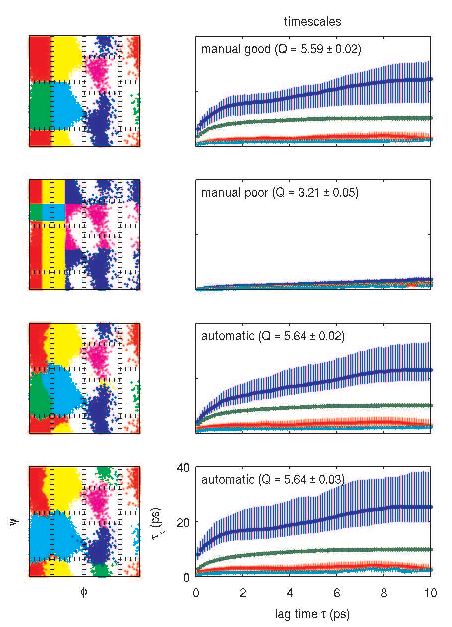
\includegraphics{chapters/automatic-state-decomposition/figures/alanine-dipeptide/alanine-dipeptide-comparison-manual-automatic.pdf}}
  \end{center}
  \caption{{\bf Comparison of manual and automatic state decompositions for alanine dipeptide.}  
  The left panels depict state partitionings, and the right panels the associated timescales (in picoseconds) as a function of lag time with uncertainties shown, as estimated from the procedure described in Section \ref{section:methods:validation}.
  Top two panels: Manual ``good'' or ``gold standard'' state decomposition from Ref.\ \cite{chodera:mms:2006} and manual ``poor'' state decomposition, where the state boundaries are grossly distorted so as to include internal kinetic barriers within the states.
  Bottom two panels: Two nearly-equivalent partitionings obtained from the automatic state decomposition algorithm.
  }
  \label{figure:alanine-dipeptide-manual-vs-automatic}
\end{figure}

The results of the automatic state decomposition algorithm applied to this reduced dataset can be seen in Figure \ref{figure:alanine-dipeptide-manual-vs-automatic}, in comparison with the ``gold standard'' manual state decomposition from Ref.\ \cite{chodera:mms:2006} and a ``poor'' manual decomposition that is expected to fail to reproduce kinetics well because its states include internal kinetic barriers\footnote{The poor partitioning was defined as follows: (1) $\phi \in [(179,-135]$, $\psi \in (98,48]$; (2) $\phi \in (-135,-60]$, $\psi \in (98,48]$; (3) $\phi \in (179,-135]$, $\psi \in (48,98]$; (4) $\phi \in (-135,-60]$, $\psi \in (48,98]$; (5) $\phi \in (-60,179]$, $\psi \in (98,-45]$; (6) $\phi \in (-60,179]$, $\psi \in (-45,98]$.  Specified intervals denote intervals on the torus, which is continuous from -180 to +180.  All torsions are specified in degrees.}.
Independent applications of the automatic method were observed to yield two distinct decompositions with metastabilities within statistical uncertainty, both of which slightly exceeded the metastability of the manual decomposition (Figure \ref{figure:alanine-dipeptide-manual-vs-automatic}, bottom two plots).
In the automatic decomposition with slightly larger metastability, six states in the same general locations as the manual ``gold standard'' decomposition are observed, though the boundaries are somewhat perturbed.
However, the timescales as a function of lag time are not significantly different from those of the manual ``gold standard'' decomposition  (Figure \ref{figure:alanine-dipeptide-manual-vs-automatic}, right) .
In the other automatic decomposition with nearly equal metastability, states 3 and 4 of the manual decomposition (numbering given in Figure \ref{figure:alanine-dipeptide-2d-pmf}) have been merged into a single state, and state 5 of the manual decomposition has been fragmented into two states.
Despite this, the timescales as a function of lag time again appear to be statistically indistinguishable from those of the ``gold standard'', suggesting that this model may have equal utility.
This suggests that the phenomenological rates may not be very sensitive to the exact choice of state boundaries after the Markov time, as recrossings will have been suppressed by this time.
The fact that this lumping does not disrupt the behavior of the model substantially is not altogether surprising, because the barrier separating states 3 and 4 is rather small, and these states act like a single state even on timescales of a few picoseconds or greater.
In contrast, the ``poor'' decomposition has extremely short timescales which do not appear to level off over the course of 10 ps.

\begin{figure}[tb]
  \begin{center}
    \resizebox{3.375in}{!}{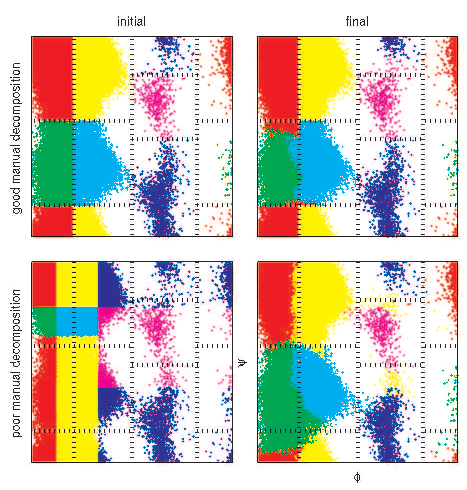
\includegraphics{chapters/automatic-state-decomposition/figures/alanine-dipeptide/alanine-dipeptide-comparison-initial-final.pdf}}  
  \end{center}
  \caption{{\bf Stability and recovery of optimal state decomposition for alanine dipeptide.}
  Top: Ten cycles of automatic state decomposition applied to a ``good'' manual partitioning (left) to yield an automatic partitioning (right).
  Bottom: Ten cycles of automatic state decomposition applied to a ``poor'' manual partitioning (left) to yield an automatic partitioning (right).
  }
  \label{figure:alanine-dipeptide-decomposition-stability}
\end{figure}

To examine the ability of the algorithm to recover optimal partitionings, the automatic state decomposition algorithm was applied to both the ``gold standard'' and ``poor'' manual decompositions (Figure \ref{figure:alanine-dipeptide-decomposition-stability}) to see whether these partitionings would be maintained over the course of subsequent iterations.
Ten iterations were conducted, with each macrostate split to ten microstates in the first iteration, rather than the entire configuration space being split into 100 states.
In both cases, the algorithm converged to nearly equivalent partitionings after ten iterations (Figure \ref{figure:alanine-dipeptide-decomposition-stability}), as verified by examination of the converged timescales (data not shown).
This suggests the method yields partitionings that are relatively stable and optimal.

From the ``poor'' manual decomposition, however, a number of conformations in manual states 5 and 6 are incorrectly grouped with state 2, though this did not significantly affect the timescales.
Further investigation showed that the algorithm never split these conformations from state 2, partly due to their comprising only 1 \% of the population of the state.
Splitting each macrostate into more microstates should alleviate this problem.
